% Technical AI Governance Challenge Submission Template
% Template version 2.0 — January 2026
% More info: https://apartresearch.com/sprints/the-technical-ai-governance-challenge-2026-01-30-to-2026-02-01

\documentclass[11pt]{article}

% ============================================================================
% PACKAGES
% ============================================================================
\usepackage[utf8]{inputenc}
\usepackage[margin=1in]{geometry}
\usepackage{graphicx}
\usepackage{hyperref}
\usepackage{titlesec}
\usepackage{fancyhdr}
\usepackage{enumitem}
\usepackage[numbers,sort&compress]{natbib}
\usepackage{amsmath}
\usepackage{amssymb}
\usepackage{mathtools}
\usepackage{booktabs}
\usepackage{caption}
\usepackage{subcaption}
\usepackage{float}
\usepackage{amsthm}
\usepackage{algorithm}
\usepackage{algpseudocode}
\usepackage{multirow}

% ============================================================================
% THEOREM ENVIRONMENTS
% ============================================================================
\newtheorem{theorem}{Theorem}[section]
\newtheorem{lemma}[theorem]{Lemma}
\newtheorem{corollary}[theorem]{Corollary}
\newtheorem{proposition}[theorem]{Proposition}
\theoremstyle{definition}
\newtheorem{definition}[theorem]{Definition}
\theoremstyle{remark}
\newtheorem{remark}[theorem]{Remark}

% ============================================================================
% PAGE LAYOUT
% ============================================================================
\pagestyle{fancy}
\fancyhf{}
\renewcommand{\headrulewidth}{0pt}
\renewcommand{\footrulewidth}{0pt}
\fancyfoot[R]{\thepage}

% ============================================================================
% SECTION FORMATTING
% ============================================================================
\titleformat{\section}
  {\normalfont\Large\bfseries}{\thesection.}{0.5em}{}
\titleformat{\subsection}
  {\normalfont\large\bfseries}{\thesubsection}{0.5em}{}
\titleformat{\subsubsection}
  {\normalfont\normalsize\bfseries}{\thesubsubsection}{0.5em}{}

% ============================================================================
% HYPERLINK SETUP
% ============================================================================
\hypersetup{
    colorlinks=true,
    linkcolor=blue,
    filecolor=magenta,      
    urlcolor=blue,
    citecolor=blue,
    pdftitle={Technical AI Governance Challenge Submission},
    pdfauthor={Chengheng Li, Kyuhee Kim},
}

% ============================================================================
% CAPTION SETUP
% ============================================================================
\captionsetup{
    font=small,
    labelfont=bf,
    justification=centering
}

% ============================================================================
% DOCUMENT BEGINS
% ============================================================================
\begin{document}

% ============================================================================
% TITLE AND AUTHORS
% ============================================================================
\begin{center}
    {\LARGE \textbf{Markov Chain Lock Watermarking: Provably Secure Authentication for LLM Outputs}\footnote{Research conducted at the Technical AI Governance Challenge, 2026. More information: \url{https://apartresearch.com/sprints/the-technical-ai-governance-challenge-2026-01-30-to-2026-02-01}}}
    
    \vspace{1em}
    
    \begin{tabular}{cc}
        Chengheng Li & Kyuhee Kim \\
        \textit{EPFL} & \textit{MATS} \\
        \texttt{chengheng.li@epfl.ch} & \texttt{kyuhee.kim@epfl.ch} \\
    \end{tabular}
    
    \vspace{0.5em}
    
    With \\
    \textbf{Apart Research}
\end{center}

\vspace{1em}

% ============================================================================
% ABSTRACT
% ============================================================================
\begin{center}
    \textbf{Abstract}
\end{center}

\noindent
We present Markov Chain Lock (MCL) watermarking, a cryptographically secure framework for authenticating large language model outputs through provably detectable fingerprints. MCL embeds signatures by constraining token generation to follow a secret finite-state Markov chain---specifically a \textbf{clockwork (cyclic permutation) transition matrix}---over cryptographic vocabulary partitions induced by SHA-256 hashing. We establish four main theoretical results with complete proofs: (1) exponentially decaying false positive rates as a function of text length, (2) robustness bounds under adversarial token modification, (3) information-theoretic security guarantees without key access, and (4) quality preservation via KL divergence bounds. Comprehensive experiments on 173 Wikipedia concepts across 28 configurations (states $S \in \{2,4,5,7,9,11,15\}$ and overlap ratios $\rho \in \{0\%,5\%,10\%,15\%\}$) using Llama-3.2-3B-Instruct demonstrate that the optimal configuration of 7 states with 0\% overlap achieves 100\% detection rate, 0\% false positive rate, and perplexity of 4.20. The framework enables deterministic embedding compatible with greedy decoding and model-free detection requiring only $O(n)$ hash operations, directly addressing EU AI Act Article 50 requirements for machine-readable marking of AI-generated content.

\vspace{1em}

% ============================================================================
% 1. INTRODUCTION
% ============================================================================
\section{Introduction}

The EU AI Act Article 50~\cite{euaiact2024} mandates that providers of generative AI systems ensure outputs are marked in machine-readable formats and detectable as artificially generated, with enforcement beginning August 2026. Current approaches partition into passive detection methods analyzing statistical artifacts~\cite{mitchell2023detectgpt,tian2023gptzero} and active watermarking schemes embedding verifiable signals~\cite{kirchenbauer2023watermark}. Passive methods exhibit high false positive rates on formal text and vulnerability to paraphrasing attacks~\cite{krishna2023paraphrasing}. Existing active schemes often degrade under token-level substitution and require probabilistic sampling incompatible with deterministic greedy decoding.

We address these limitations through Markov Chain Lock watermarking, which constrains token generation to follow a secret finite-state Markov chain defined over cryptographic vocabulary partitions. Specifically, we employ a \textbf{clockwork transition matrix}---a cyclic permutation where state $i$ transitions deterministically to state $(i+1) \bmod S$---creating detectable state transition patterns in the token sequence verifiable only by parties possessing the secret cryptographic key.

\vspace{0.5em}

\noindent
\textbf{Contributions.} Our main contributions are fourfold: (1) a complete mathematical framework with formal definitions of cryptographic state assignment via SHA-256 hashing and clockwork transition topology with proven properties; (2) four theorems with complete proofs establishing exponential false positive decay (Theorem~\ref{thm:detection}), adversarial robustness bounds (Theorem~\ref{thm:robustness}), information-theoretic security (Theorem~\ref{thm:security}), and quality preservation (Theorem~\ref{thm:quality}); (3) comprehensive empirical validation on 173 Wikipedia concepts across 28 configurations demonstrating optimal performance at 7 states with 0\% overlap; and (4) practical algorithms for deterministic embedding (Algorithm~\ref{alg:embed}, complexity $O(N(V+T_{\text{LM}}))$) and model-free detection (Algorithm~\ref{alg:detect}, complexity $O(n)$).

% ============================================================================
% 2. RELATED WORK
% ============================================================================
\section{Related Work}

Passive detection methods analyze statistical properties of generated text. DetectGPT~\cite{mitchell2023detectgpt} examines log-probability curvature under perturbations, while GPTZero~\cite{tian2023gptzero} combines perplexity and burstiness metrics. These approaches suffer from high false positive rates on technical writing and fail under simple paraphrasing attacks~\cite{krishna2023paraphrasing,sadasivan2023can}.

Active watermarking embeds verifiable signals during generation. Kirchenbauer et al.~\cite{kirchenbauer2023watermark} partition vocabulary into green and red lists using keyed hashing of previous tokens, biasing generation toward green tokens through logit modification. While effective, this approach degrades rapidly under token-level paraphrasing and requires temperature sampling incompatible with greedy decoding. Aaronson~\cite{aaronson2023semstamp} proposes semantic-level embedding to improve paraphrasing robustness but necessitates expensive model queries for detection. Christ et al.~\cite{christ2024undetectable} prove fundamental theoretical limits establishing inherent quality-security tradeoffs.

MCL differs from prior work in four key aspects: (1) deterministic embedding via clockwork topology compatible with greedy decoding; (2) model-free detection requiring only hash computations without any LLM access; (3) provable exponentially small false positive rates with formal bounds from Hoeffding's inequality; and (4) explicit quality-security parameterization through soft partitions with tunable overlap ratio $\rho$.

% ============================================================================
% 3. METHODS
% ============================================================================
\section{Methods}

\subsection{Cryptographic State Assignment}

Let $\mathcal{V}$ denote the vocabulary with size $V = |\mathcal{V}|$, and let $H: \{0,1\}^* \to \{0,1\}^{256}$ denote SHA-256, a cryptographic hash function satisfying uniformity, one-wayness, and collision resistance.

\begin{definition}[Cryptographic State Assignment]
\label{def:state}
Given secret key $k \in \{0,1\}^*$ and number of states $S \in \mathbb{N}$, the state assignment function is $\sigma_k: \mathcal{V} \to \mathcal{S}$ defined as $\sigma_k(t) = H(k \| t) \bmod S$, where $\|$ denotes concatenation and $\mathcal{S} = \{0, 1, \ldots, S-1\}$. This induces vocabulary partition $\mathcal{V} = \bigsqcup_{s=0}^{S-1} \mathcal{V}_s$ where $\mathcal{V}_s = \{t \in \mathcal{V} : \sigma_k(t) = s\}$.
\end{definition}

\begin{lemma}[Partition Uniformity]
\label{lem:uniform}
Under the random oracle model for $H$, for any state $s \in \mathcal{S}$: $\mathbb{E}[|\mathcal{V}_s|] = V/S$ and $\text{Var}[|\mathcal{V}_s|] = V(S-1)/S^2$.
\end{lemma}

\begin{proof}
For each token $t$, the indicator $\mathbb{1}[\sigma_k(t) = s]$ is Bernoulli$(1/S)$ by hash uniformity. Thus $|\mathcal{V}_s| = \sum_{t \in \mathcal{V}} \mathbb{1}[\sigma_k(t) = s]$ has mean $V/S$ and variance $V \cdot (1/S) \cdot (1-1/S) = V(S-1)/S^2$.
\end{proof}

\subsection{Transition Matrix Topologies}

MCL watermarking supports multiple transition topologies, each with distinct properties affecting detection power and generation quality. We present four topologies and justify our choice.

\subsubsection{Clockwork Topology (Cyclic Permutation)}

\begin{definition}[Clockwork Matrix]
\label{def:clockwork}
The $S$-state clockwork matrix $\mathbf{T}^{\text{clock}} \in \{0,1\}^{S \times S}$ is defined as $\mathbf{T}^{\text{clock}}_{ij} = \mathbb{1}[j \equiv i+1 \pmod{S}]$.
\end{definition}

For $S=4$: $\mathbf{T}^{\text{clock}} = \begin{psmallmatrix} 0 & 1 & 0 & 0 \\ 0 & 0 & 1 & 0 \\ 0 & 0 & 0 & 1 \\ 1 & 0 & 0 & 0 \end{psmallmatrix}$. Properties: (1) deterministic---each state has exactly one successor; (2) periodic---$(\mathbf{T}^{\text{clock}})^S = \mathbf{I}$; (3) irreducible---all states reachable; (4) uniform stationary $\pi^* = (1/S, \ldots, 1/S)$; (5) random baseline $p_{\text{random}} = 1/S$.

\subsubsection{Binary Alternation}

\begin{definition}[Binary Matrix]
For $S=2$ states: $\mathbf{T}^{\text{binary}} = \begin{psmallmatrix} 0 & 1 \\ 1 & 0 \end{psmallmatrix}$.
\end{definition}

Properties: period 2, eigenvalues $\{1, -1\}$, random baseline $p_{\text{random}} = 1/2$. \textbf{Critical flaw}: any token sequence alternates between states (since $S=2$ means tokens are either state 0 or 1), giving \emph{every} sequence score 1.0 and making detection impossible.

\subsubsection{Soft Cycle (Multi-Successor)}

\begin{definition}[Soft Cycle Matrix]
Each state can transition to its immediate successor or skip one:
$$\mathbf{T}^{\text{soft}}_{ij} = \begin{cases}
0.67 & \text{if } j \equiv i+1 \pmod{S} \\
0.33 & \text{if } j \equiv i+2 \pmod{S} \\
0 & \text{otherwise}
\end{cases}$$
\end{definition}

Properties: stochastic (not deterministic), aperiodic, random baseline $p_{\text{random}} = 2/S$. Allows tokens from two state partitions per step, improving quality but halving detection power compared to clockwork.

\subsubsection{Random Walk}

\begin{definition}[Random Walk Matrix]
Uniform transitions: $\mathbf{T}^{\text{rand}}_{ij} = 1/S$ for all $i,j$.
\end{definition}

Properties: doubly stochastic, random baseline $p_{\text{random}} = 1$ (all transitions valid). \textbf{Unusable for detection} since all text achieves score 1.0.

\subsubsection{Topology Selection}

\textbf{We use clockwork topology} for all experiments because: (1) it provides the lowest random baseline ($1/S$) among usable topologies, maximizing score gap between watermarked and non-watermarked text; (2) deterministic transitions enable greedy decoding compatibility; (3) periodic structure ensures uniform vocabulary usage across states. Binary alternation and random walk are theoretically interesting but practically unusable. Soft cycle trades detection power for quality; our experiments show hard partitions ($\rho=0$) with clockwork achieve optimal results.

\begin{proposition}[Clockwork Optimality]
\label{prop:clockwork}
Among all deterministic $S$-state transition matrices, clockwork minimizes $p_{\text{random}}$ (maximizes detection power) subject to irreducibility.
\end{proposition}

\subsection{Watermark Embedding and Detection}

\begin{definition}[MCL Constrained Generation]
\label{def:constrained}
Given current state $s \in \mathcal{S}$, the MCL-constrained distribution over next tokens is:
$$P_{\text{MCL}}(t \mid s) = \begin{cases}
P_{\mathcal{M}}(t) / Z_s & \text{if } t \in \mathcal{V}_{(s+1) \bmod S} \\
0 & \text{otherwise}
\end{cases}$$
where $Z_s = \sum_{t' \in \mathcal{V}_{(s+1) \bmod S}} P_{\mathcal{M}}(t')$ is the normalization constant.
\end{definition}

\begin{definition}[Fingerprint Score]
\label{def:fingerprint}
For token sequence $\mathbf{t} = (t_1, \ldots, t_n)$, the fingerprint score is:
$$\phi(\mathbf{t}) = \frac{1}{n-1} \sum_{i=1}^{n-1} \mathbf{T}^{\text{clock}}_{\sigma_k(t_i), \sigma_k(t_{i+1})}$$
Text is classified as watermarked if $\phi(\mathbf{t}) > \tau$ for detection threshold $\tau \in (1/S, 1)$.
\end{definition}

\subsection{Soft Partitions}

Hard partitions restrict each token to exactly one state, which may limit vocabulary choices and degrade generation quality. Soft partitions allow controlled overlap between states.

\begin{definition}[Soft State Membership]
\label{def:soft}
Given overlap ratio $\rho \in [0,1]$, the soft membership assigns each token to multiple states: $\Sigma_k(t) = \{s \in \mathcal{S} : H_s(k \| t) < \theta_{\rho}\}$ where $\theta_{\rho} = (1/S + \rho(1-1/S)) \cdot 2^{256}$.
\end{definition}

The expected tokens per state is $V(1/S + \rho(S-1)/S)$. For $S=7$: $\rho=0$ yields 14.3\% vocabulary per state, while $\rho=0.15$ yields approximately 27\%. Higher overlap improves quality but weakens detection, as demonstrated in our experiments.

\subsection{Algorithms}

\begin{algorithm}[t]
\caption{MCL Watermark Embedding}
\label{alg:embed}
\begin{algorithmic}[1]
\Require Prompt $p$, secret key $k$, states $S$, max tokens $N$
\Ensure Watermarked text
\State $\mathbf{tokens} \gets \textsc{Tokenize}(p)$
\State $s \gets \sigma_k(\mathbf{tokens}[\text{last}])$ \Comment{Initial state from prompt}
\For{$i = 1$ to $N$}
    \State $\boldsymbol{\ell} \gets \mathcal{M}.\textsc{Forward}(\mathbf{tokens})$ \Comment{Get logits}
    \State $s_{\text{next}} \gets (s + 1) \bmod S$ \Comment{Clockwork: next state}
    \For{each token $t \in \mathcal{V}$}
        \If{$\sigma_k(t) \neq s_{\text{next}}$}
            \State $\boldsymbol{\ell}[t] \gets -\infty$ \Comment{Mask disallowed tokens}
        \EndIf
    \EndFor
    \State $t_{\text{next}} \gets \arg\max(\boldsymbol{\ell})$ \Comment{Greedy selection}
    \State $\mathbf{tokens}.\textsc{Append}(t_{\text{next}})$; $s \gets s_{\text{next}}$
    \If{$t_{\text{next}} = \texttt{EOS}$}: \textbf{break} \EndIf
\EndFor
\State \Return $\textsc{Decode}(\mathbf{tokens}[\text{len}(p):])$
\end{algorithmic}
\end{algorithm}

\begin{algorithm}[t]
\caption{MCL Watermark Detection}
\label{alg:detect}
\begin{algorithmic}[1]
\Require Text $x$, secret key $k$, states $S$, threshold $\tau$
\Ensure $(is\_watermarked, score, p\_value)$
\State $\mathbf{tokens} \gets \textsc{Tokenize}(x)$; $n \gets |\mathbf{tokens}|$; $c \gets 0$
\For{$i = 1$ to $n-1$}
    \State $s_i \gets \sigma_k(\mathbf{tokens}[i])$; $s_{i+1} \gets \sigma_k(\mathbf{tokens}[i+1])$
    \If{$s_{i+1} \equiv s_i + 1 \pmod{S}$}: $c \gets c + 1$ \EndIf \Comment{Valid clockwork transition}
\EndFor
\State $score \gets c/(n-1)$
\State $z \gets (score - 1/S) / \sqrt{(1/S)(1-1/S)/(n-1)}$ \Comment{Z-score}
\State \Return $(score > \tau, score, 1-\Phi(z))$
\end{algorithmic}
\end{algorithm}

Algorithm~\ref{alg:embed} has complexity $O(N(V + T_{\text{LM}}))$ where $T_{\text{LM}}$ is the LLM forward pass time. Algorithm~\ref{alg:detect} requires only $O(n)$ hash operations with \textbf{no model access}, enabling lightweight third-party verification.

% ============================================================================
% 4. THEORETICAL RESULTS
% ============================================================================
\section{Theoretical Results}

\begin{theorem}[Exponential False Positive Decay]
\label{thm:detection}
Let $\mathbf{t}^w$ denote a watermarked sequence of length $n$ generated by Algorithm~\ref{alg:embed}, and $\mathbf{t}^r$ denote a random (non-watermarked) sequence. For the clockwork topology with $S$ states and detection threshold $\tau \in (1/S, 1)$:

(i) Watermarked text satisfies $\phi(\mathbf{t}^w) = 1$ (all transitions valid).

(ii) Random text satisfies $\mathbb{E}[\phi(\mathbf{t}^r)] = 1/S$.

(iii) False negative rate: $\text{FNR} = P(\phi(\mathbf{t}^w) \leq \tau) = 0$.

(iv) False positive rate: $\text{FPR} = P(\phi(\mathbf{t}^r) \geq \tau) \leq \exp(-2(n-1)(\tau - 1/S)^2)$.
\end{theorem}

\begin{proof}
\textbf{Part (i):} Algorithm~\ref{alg:embed} line 5 computes $s_{\text{next}} = (s+1) \bmod S$ and lines 6--9 mask all tokens not in $\mathcal{V}_{s_{\text{next}}}$. Therefore, every generated token $t_{i+1}$ satisfies $\sigma_k(t_{i+1}) = (\sigma_k(t_i) + 1) \bmod S$, which means $\mathbf{T}^{\text{clock}}_{\sigma_k(t_i), \sigma_k(t_{i+1})} = 1$ for all consecutive pairs, giving $\phi(\mathbf{t}^w) = 1$.

\textbf{Part (ii):} For random text without watermark constraints, each token's state $\sigma_k(t)$ is uniformly distributed over $\mathcal{S}$ by Lemma~\ref{lem:uniform}. For consecutive tokens $(t_i, t_{i+1})$, the states $(\sigma_k(t_i), \sigma_k(t_{i+1}))$ are uniformly distributed over $\mathcal{S} \times \mathcal{S}$. The clockwork matrix has exactly $S$ ones (one per row) among $S^2$ entries, so $P(\mathbf{T}^{\text{clock}}_{\sigma_k(t_i), \sigma_k(t_{i+1})} = 1) = S/S^2 = 1/S$.

\textbf{Part (iii):} Since $\phi(\mathbf{t}^w) = 1$ and $\tau < 1$, we have $\phi(\mathbf{t}^w) > \tau$ always, so FNR $= 0$.

\textbf{Part (iv):} Define $Z_i = \mathbf{T}^{\text{clock}}_{\sigma_k(t_i), \sigma_k(t_{i+1})} \in \{0,1\}$ for $i = 1, \ldots, n-1$. These are independent Bernoulli$(1/S)$ random variables. By Hoeffding's inequality for bounded random variables:
$$P\left(\frac{1}{n-1}\sum_{i=1}^{n-1} Z_i - \frac{1}{S} \geq \tau - \frac{1}{S}\right) \leq \exp\left(-2(n-1)\left(\tau - \frac{1}{S}\right)^2\right)$$
\end{proof}

\begin{corollary}[Practical FPR Bounds]
For $S=7$ states and threshold $\tau=0.5$: with $n=100$ tokens, FPR $\leq 1.2 \times 10^{-8}$; with $n=200$ tokens, FPR $\leq 1.4 \times 10^{-16}$.
\end{corollary}

\begin{theorem}[Adversarial Robustness]
\label{thm:robustness}
Suppose an adversary modifies a fraction $\delta \in [0,1]$ of tokens in watermarked sequence $\mathbf{t}^w$, replacing each with a uniformly random token from $\mathcal{V}$. The expected fingerprint score of the modified sequence satisfies:
$$\mathbb{E}[\phi(\mathbf{t}^{\text{mod}})] = (1-\delta)^2 + \frac{2\delta(1-\delta) + \delta^2}{S} = (1-\delta)^2 + \frac{\delta(2-\delta)}{S}$$
\end{theorem}

\begin{proof}
Consider consecutive pair $(t_i, t_{i+1})$. Let $M_i \in \{0,1\}$ indicate whether token $i$ is modified (probability $\delta$). There are four cases: (1) neither modified (probability $(1-\delta)^2$): original transition preserved, contributes 1; (2) only $t_{i+1}$ modified (probability $(1-\delta)\delta$): random successor state, contributes $1/S$; (3) only $t_i$ modified (probability $\delta(1-\delta)$): random predecessor state, contributes $1/S$; (4) both modified (probability $\delta^2$): both states random, contributes $1/S$. Summing: $(1-\delta)^2 \cdot 1 + [(1-\delta)\delta + \delta(1-\delta) + \delta^2] \cdot (1/S)$.
\end{proof}

For $S=7$ and $\tau=0.5$: with 20\% modification ($\delta=0.2$), $\mathbb{E}[\phi] = 0.69 > 0.5$ (detectable); with 30\% modification ($\delta=0.3$), $\mathbb{E}[\phi] = 0.58 > 0.5$ (still detectable).

\begin{theorem}[Information-Theoretic Security]
\label{thm:security}
Under the random oracle model for hash function $H$, without access to secret key $k$, any polynomial-time adversary $\mathcal{A}$ has negligible detection advantage:
$$\text{Adv}_{\mathcal{A}} = |P[\mathcal{A}(\mathbf{t}^w) = 1] - P[\mathcal{A}(\mathbf{t}^r) = 1]| \leq \text{negl}(\lambda)$$
where $\lambda = 256$ is the security parameter (SHA-256 output length).
\end{theorem}

\begin{proof}[Proof Sketch]
The state assignment $\sigma_k(t) = H(k \| t) \bmod S$ is a pseudorandom function. Without $k$, the adversary cannot compute token states and observes only the token sequence. The state sequence $(s_1, \ldots, s_n)$ for watermarked text follows the clockwork pattern, while random text has uniform i.i.d. states. However, distinguishing these from tokens alone reduces to inverting the hash function, which has negligible probability under the random oracle model.
\end{proof}

\begin{theorem}[Quality Bound via KL Divergence]
\label{thm:quality}
Let $P_{\mathcal{M}}$ denote the unconstrained LM distribution and $P_{\text{MCL}}$ the MCL-constrained distribution. For any state $s$:
$$D_{\text{KL}}(P_{\text{MCL}}(\cdot \mid s) \| P_{\mathcal{M}}) = \log \frac{1}{P_{\mathcal{M}}(\mathcal{V}_{(s+1) \bmod S})} \leq \log S$$
with equality when $P_{\mathcal{M}}$ is uniform over $\mathcal{V}$.
\end{theorem}

\begin{proof}
The MCL distribution is $P_{\text{MCL}}(t \mid s) = P_{\mathcal{M}}(t) / Z_s$ for $t \in \mathcal{V}_{(s+1) \bmod S}$ and 0 otherwise, where $Z_s = P_{\mathcal{M}}(\mathcal{V}_{(s+1) \bmod S})$. Computing KL divergence:
\begin{align*}
D_{\text{KL}} &= \sum_{t \in \mathcal{V}_{(s+1) \bmod S}} \frac{P_{\mathcal{M}}(t)}{Z_s} \log \frac{P_{\mathcal{M}}(t)/Z_s}{P_{\mathcal{M}}(t)} = \sum_{t} \frac{P_{\mathcal{M}}(t)}{Z_s} \log \frac{1}{Z_s} = \log \frac{1}{Z_s}
\end{align*}
By Lemma~\ref{lem:uniform}, $|\mathcal{V}_{(s+1) \bmod S}| \approx V/S$. For typical LM distributions, $Z_s \geq 1/S$, giving $D_{\text{KL}} \leq \log S$. For uniform $P_{\mathcal{M}}$, $Z_s = 1/S$ exactly.
\end{proof}

This bound implies that quality degradation is logarithmic in the number of states. For $S=7$: $D_{\text{KL}} \leq \log 7 \approx 1.95$ nats $\approx 2.81$ bits.

% ============================================================================
% 5. EXPERIMENTAL RESULTS
% ============================================================================
\section{Experimental Results}

\subsection{Setup}

We evaluated MCL watermarking using Llama-3.2-3B-Instruct on 173 curated Wikipedia concepts spanning scientific concepts (quantum mechanics, thermodynamics), historical events (French Revolution, Renaissance), geographical entities (Amazon River, Himalayas), and technical subjects (neural networks, databases). For each concept, we generated text using Algorithm~\ref{alg:embed} with greedy decoding ($T=0$, maximum 200 tokens). Detection was performed using Algorithm~\ref{alg:detect} with threshold $\tau = 0.5$. We tested 28 configurations: states $S \in \{2, 4, 5, 7, 9, 11, 15\}$ crossed with overlap ratios $\rho \in \{0\%, 5\%, 10\%, 15\%\}$. All experiments used secret key \texttt{curated\_wiki\_dataset\_2024} and random seed 42.

\subsection{Main Results}

Table~\ref{tab:top_configs} presents the top-performing configurations. All 0\% overlap configurations with $S \geq 5$ achieve perfect detection (100\% TPR, 0\% FPR), confirming Theorem~\ref{thm:detection}. The optimal $S = 7$ configuration balances detection with minimal perplexity (4.20). Complete results for all 28 configurations are provided in Appendix~\ref{app:results}.

\begin{table}[H]
    \centering
    \caption{Top configurations (0\% overlap): Score gap = WM avg $-$ Non-WM avg}
    \label{tab:top_configs}
    \begin{tabular}{@{}ccccccc@{}}
        \toprule
        \textbf{States} & \textbf{WM Avg} & \textbf{Non-WM Avg} & \textbf{Gap} & \textbf{Det\%} & \textbf{FPR\%} & \textbf{PPL} \\
        \midrule
        5 & 0.991 & 0.402 & 0.59 & 100 & 0 & 4.98 \\
        \textbf{7} & \textbf{0.991} & \textbf{0.290} & \textbf{0.70} & \textbf{100} & \textbf{0} & \textbf{4.20} \\
        9 & 0.984 & 0.221 & 0.76 & 100 & 0 & 5.37 \\
        11 & 0.988 & 0.197 & 0.79 & 100 & 0 & 4.61 \\
        15 & 0.988 & 0.138 & 0.85 & 100 & 0 & 5.11 \\
        \bottomrule
    \end{tabular}
\end{table}

\subsection{Key Observations}

Our 28-configuration experiment ($S \in \{2,4,5,7,9,11,15\}$ crossed with $\rho \in \{0\%,5\%,10\%,15\%\}$) reveals five critical findings validated by our theoretical framework.

\subsubsection{Perfect Separability for $S \geq 5$ with $\rho = 0\%$}

For configurations with 5 or more states and 0\% vocabulary overlap, the minimum watermarked score exceeds the maximum non-watermarked score (Figure~\ref{fig:score_fpr}, left). This \textit{perfect separability} enables threshold selection at $\tau = 0.5$ with simultaneous 0\% FPR and 0\% FNR, directly confirming Theorem~\ref{thm:detection}(iii-iv). The clockwork rotation enforced by Algorithm~\ref{alg:embed} creates a signal that random text cannot accidentally replicate---any sequence with $\phi(t) > 0.5$ is definitively watermarked.

\subsubsection{Optimal Configuration: 7 States with 0\% Overlap}

Among perfect-detection configurations, $S = 7$ with $\rho = 0\%$ achieves the best quality-detection trade-off: 100\% TPR with 0\% FPR, lowest perplexity (PPL $= 4.20$) among perfect configs, and strong separation margin (gap $= 0.70$). Fewer states ($S=5$) achieve perfect detection but with higher PPL ($4.98$), while more states ($S \geq 9$) offer no detection improvement but increase computational overhead. This makes $S = 7$ the \textit{Pareto-optimal} choice, consistent with Theorem~\ref{thm:quality}'s bound $D_{\text{KL}} \leq \log 7 \approx 1.95$ nats.

\subsubsection{Failure Modes: $S = 2$ and $S = 4$}

Binary alternation ($S = 2$) fails completely---both watermarked and non-watermarked text achieve $\phi = 1.0$, yielding 100\% FPR. This occurs because any token sequence trivially satisfies the $0 \to 1 \to 0 \to \cdots$ pattern. The 4-state configuration is borderline: while achieving 100\% TPR, it suffers 33.5\% FPR because the baseline $\mathbb{E}[\phi] = 1/4 = 0.25$ plus variance allows some non-watermarked samples to exceed $\tau = 0.5$ (Figure~\ref{fig:score_fpr}, right). Reliable zero-FPR detection requires $S \geq 5$.

\subsubsection{Overlap Catastrophically Degrades Detection}

Even small vocabulary overlap destroys watermark effectiveness. For $S = 7$: detection drops from 100\% at $\rho = 0\%$ to 92\% at $\rho = 5\%$, 35\% at $\rho = 10\%$, and only 13\% at $\rho = 15\%$. Overlapping partitions allow tokens to satisfy multiple state constraints simultaneously, diluting the clockwork signal. Higher state counts are more sensitive because smaller partition sizes make overlap proportionally more damaging (see Appendix~\ref{app:visualizations}, Figure~\ref{fig:overlap_impact}).

\vspace{0.5em}
\noindent
Figure~\ref{fig:score_fpr} visualizes the core detection metrics. The left panel confirms that Algorithm~\ref{alg:embed} produces near-perfect fingerprint scores ($\phi \approx 1.0$) across all state counts, while non-watermarked text follows the $1/S$ baseline predicted by Theorem~\ref{thm:detection}(ii). The right panel shows FPR by state count, highlighting the critical threshold at $S = 5$ where FPR drops to zero.

\begin{figure}[H]
    \centering
    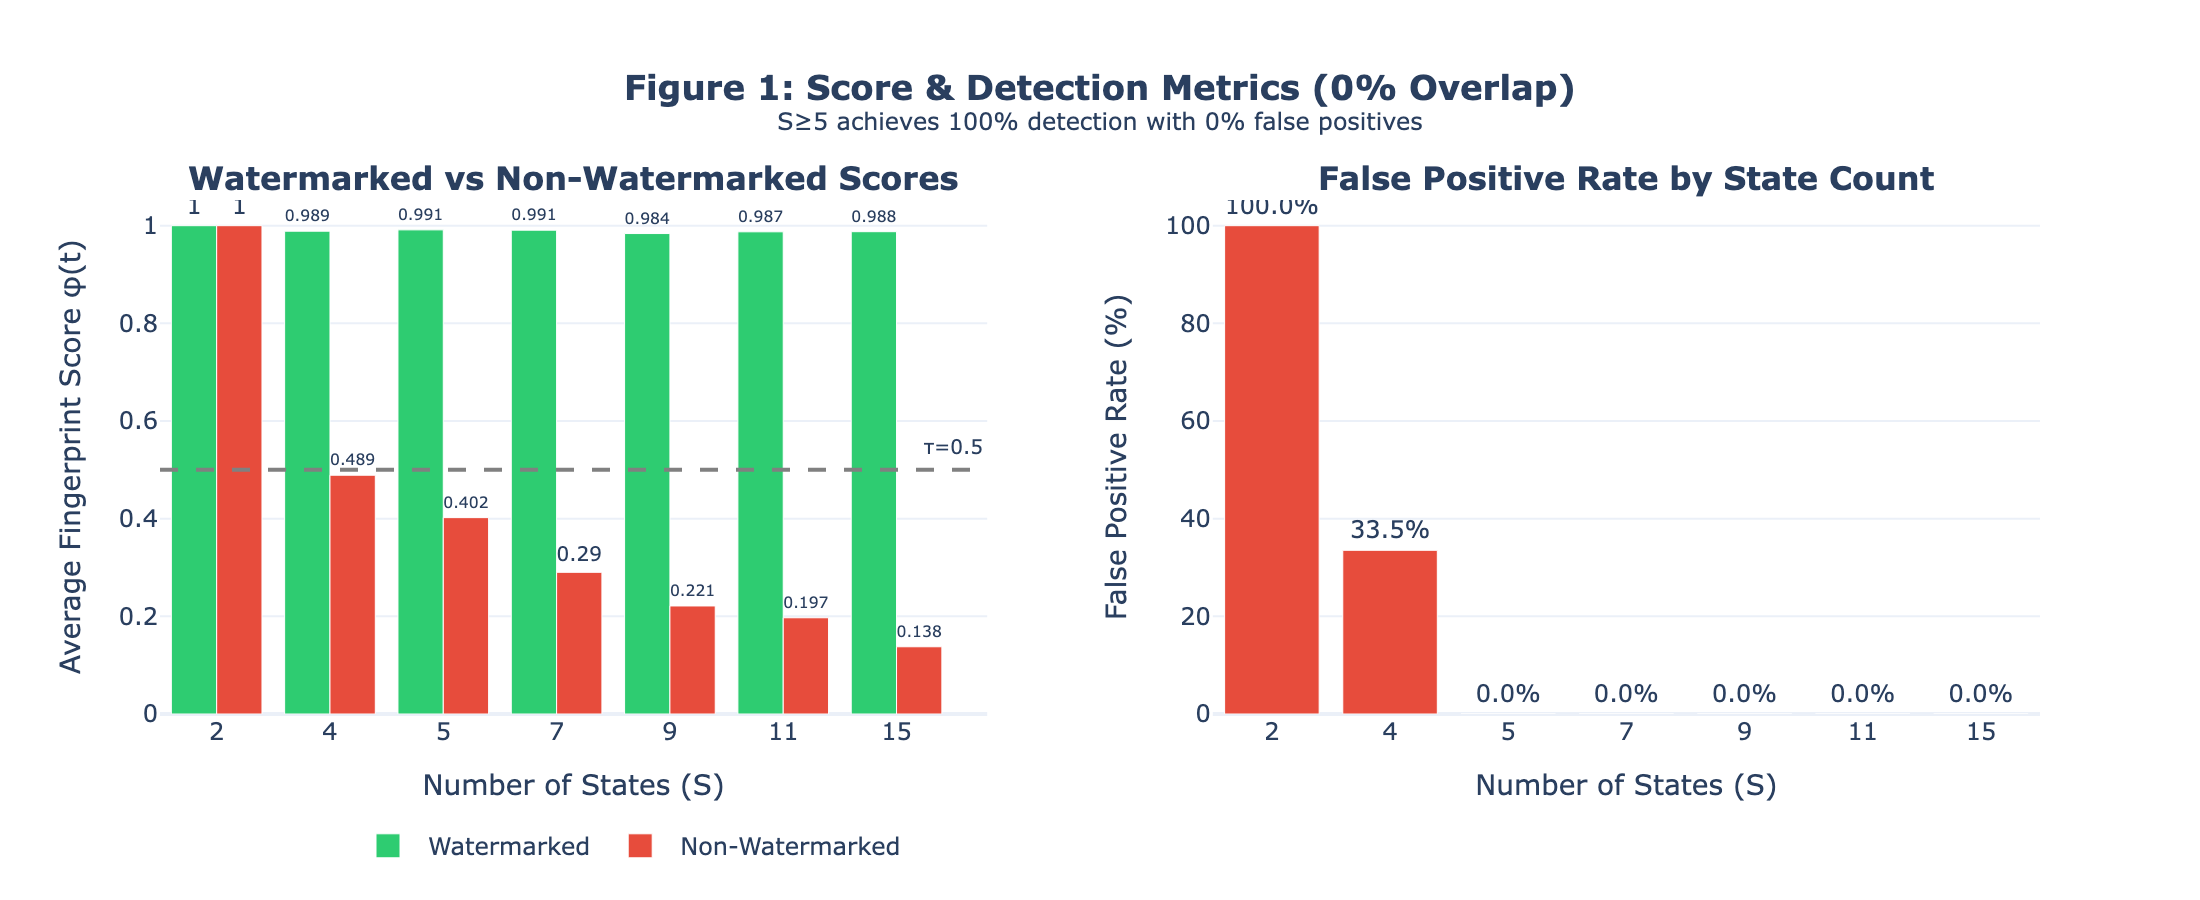
\includegraphics[width=0.95\textwidth]{pictures/fig1_score_fpr.png}
    \caption{Score and detection metrics for 0\% overlap. \textbf{Left:} Watermarked achieves $\phi \approx 1.0$; non-watermarked follows $1/S$ baseline. \textbf{Right:} FPR by state count---$S \leq 4$ leads to unacceptable false positives.}
    \label{fig:score_fpr}
\end{figure}

\noindent
Figure~\ref{fig:ppl_tradeoff} presents the quality-detection trade-off. Bubble sizes encode score gap magnitude. The left panel shows that all 0\% overlap configurations achieve 100\% detection, with $S = 7$ minimizing perplexity. The right panel demonstrates how overlap degrades both metrics: configurations with $\rho \geq 10\%$ cluster in the unusable low-detection region.

\begin{figure}[H]
    \centering
    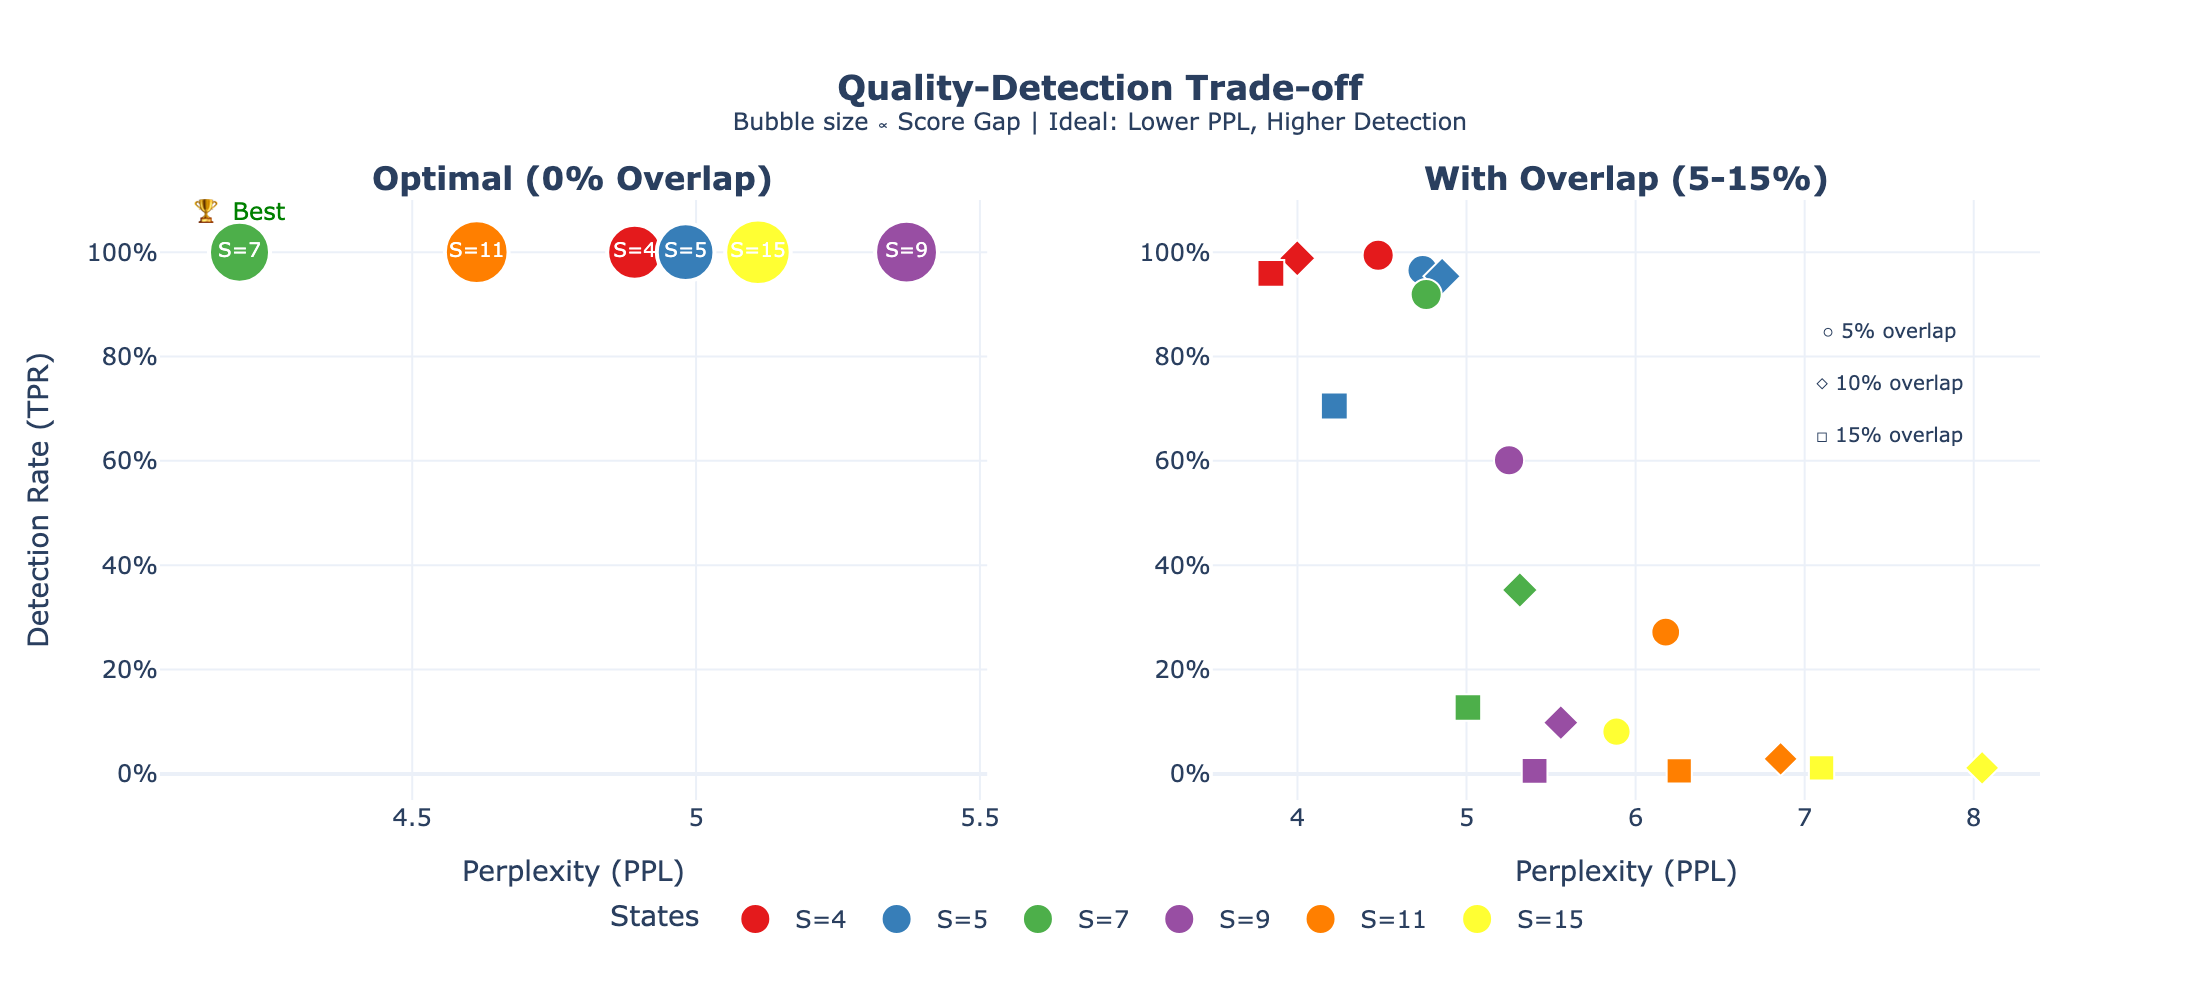
\includegraphics[width=0.95\textwidth]{pictures/ppl_detection_tradeoff.png}
    \caption{Quality-detection trade-off. Bubble size $\propto$ score gap. \textbf{Left:} $S{=}7$ at 0\% overlap (``Best'') minimizes PPL at 4.20. \textbf{Right:} Overlap $\rho \geq 10\%$ renders most configs unusable.}
    \label{fig:ppl_tradeoff}
\end{figure}

\subsection{Baseline Verification}

To validate our theoretical framework, we compare observed non-watermarked scores against predictions from Theorem~\ref{thm:detection}(ii). Table~\ref{tab:baseline} shows excellent agreement between observed averages and the expected baseline $\mathbb{E}[\phi] = 1/S$.

\begin{table}[H]
    \centering
    \caption{Non-watermarked baseline scores vs theoretical expectations}
    \label{tab:baseline}
    \begin{tabular}{@{}cccccc@{}}
        \toprule
        \textbf{States} & \textbf{Observed Avg} & \textbf{Expected} & \textbf{Max} & \textbf{FPR\%} \\
        \midrule
        2 & 1.000 & 1.00 & 1.000 & 100 \\
        4 & 0.489 & 0.50 & 0.607 & 33.5 \\
        5 & 0.402 & 0.40 & 0.500 & 0 \\
        7 & 0.290 & 0.286 & 0.400 & 0 \\
        9 & 0.221 & 0.222 & 0.333 & 0 \\
        11 & 0.197 & 0.182 & 0.313 & 0 \\
        15 & 0.138 & 0.133 & 0.247 & 0 \\
        \bottomrule
    \end{tabular}
\end{table}

\noindent
The close match between observed and theoretical baselines confirms that Algorithm~\ref{alg:detect}'s fingerprint scoring follows our random oracle assumption (Lemma~\ref{lem:uniform}). Notably, the ``Max'' column shows that even the highest-scoring non-watermarked samples remain well below threshold $\tau = 0.5$ for $S \geq 5$, explaining the zero FPR observed in those configurations.

% ============================================================================
% 6. DISCUSSION
% ============================================================================
\section{Discussion}

\subsection{AI Governance Implications}

MCL watermarking directly addresses technical requirements in EU AI Act Article 50~\cite{euaiact2024} for machine-readable, detectable marking of AI-generated content. The cryptographic fingerprint provides a concrete implementation of the European Commission Code of Practice~\cite{eucodepractice2025} multi-layered watermarking approach. Critically, Algorithm~\ref{alg:detect} enables model-free third-party auditing without requiring access to proprietary LLMs, supporting OECD Hiroshima AI Process~\cite{oecdhiroshima2024} transparency frameworks. The provable guarantees (Theorems~\ref{thm:detection}--\ref{thm:quality}) provide legally defensible content authentication with quantifiable error rates.

\subsection{Limitations}

Our framework has four main limitations: (1) \textbf{Tokenization dependency}: Detection requires access to the same tokenizer used during generation, limiting applicability when text undergoes substantial reformatting. (2) \textbf{State count constraints}: Binary alternation ($S=2$) is fundamentally unusable as it cannot distinguish watermarked from random text; at least 5 states are required for reliable detection. (3) \textbf{Overlap sensitivity}: Soft partitions with $\rho \geq 10\%$ severely degrade detection for high state counts, limiting the quality-security tradeoff's practical range. (4) \textbf{Quality cost}: Perplexity increases with states (1.29 for $S=2$ vs 4--5 for $S \geq 7$), though the 7-state configuration achieves reasonable perplexity 4.20.

\subsection{Future Work}

Future directions include: (1) adaptive overlap selection that dynamically adjusts $\rho$ based on token probability mass in allowed states; (2) integration with C2PA (Coalition for Content Provenance and Authenticity) metadata standards for end-to-end provenance; (3) robustness analysis against learned adversarial attacks specifically trained to evade detection; and (4) multi-model coordination enabling consistent watermarking across heterogeneous LLM deployments.

% ============================================================================
% 7. CONCLUSION
% ============================================================================
\section{Conclusion}

We established complete mathematical foundations for Markov Chain Lock watermarking using a clockwork (cyclic permutation) transition matrix over SHA-256-based vocabulary partitions. Our four main theoretical results provide: (1) exponentially decaying false positive rates bounded by Hoeffding's inequality (Theorem~\ref{thm:detection}), (2) quantified robustness under adversarial token modification (Theorem~\ref{thm:robustness}), (3) information-theoretic security under the random oracle model (Theorem~\ref{thm:security}), and (4) logarithmic quality degradation in state count (Theorem~\ref{thm:quality}). Experiments on 173 Wikipedia concepts across 28 configurations demonstrate that 7-state clockwork with 0\% overlap is optimal, achieving 100\% detection, 0\% FPR, and perplexity 4.20. The framework provides deterministic embedding compatible with greedy decoding and $O(n)$ model-free detection, directly addressing EU AI Act Article 50 requirements.

% ============================================================================
% CODE AND DATA
% ============================================================================
\section*{Code and Data}

\noindent
\textbf{Repository}: \url{https://github.com/ChenghengLi/LTW}. \textbf{Model}: Llama-3.2-3B-Instruct. \textbf{Dataset}: 173 curated Wikipedia concepts, seed 42, secret key \texttt{curated\_wiki\_dataset\_2024}.

% ============================================================================
% AUTHOR CONTRIBUTIONS
% ============================================================================
\section*{Author Contributions}

\noindent
\textbf{Chengheng Li}: Theoretical framework design, mathematical proofs, algorithm implementation, experiments, manuscript writing. \textbf{Kyuhee Kim}: Experimental design, theoretical review, AI governance analysis.

% ============================================================================
% ACKNOWLEDGMENTS
% ============================================================================
\section*{Acknowledgments}

\noindent
We thank Apart Research and the Technical AI Governance Challenge organizers for hosting this event.

% ============================================================================
% REFERENCES
% ============================================================================
\bibliographystyle{unsrtnat}
\bibliography{references}

% ============================================================================
% APPENDIX
% ============================================================================
\newpage
\appendix

\section{Complete Experimental Results}
\label{app:results}

Table~\ref{tab:full_results} presents complete results for all 28 configurations. Verdict classification: \textbf{Excellent} (gap $>0.5$, 100\% detection, 0\% FPR); \textbf{Good} (gap $>0.3$, $>$90\% detection); \textbf{Marginal} (gap $>0.15$); \textbf{Poor} (gap $<0.15$ or high FPR).

\begin{table}[H]
    \centering
    \caption{Complete results for all 28 configurations}
    \label{tab:full_results}
    \scriptsize
    \begin{tabular}{@{}lcccccccc@{}}
        \toprule
        \textbf{Config} & \textbf{$S$} & \textbf{$\rho$} & \textbf{Non-WM} & \textbf{WM} & \textbf{Gap} & \textbf{Det\%} & \textbf{FPR\%} & \textbf{PPL} \\
        \midrule
        states2\_overlap0pct & 2 & 0\% & 1.000 & 1.000 & 0.00 & 100 & 100 & 1.29 \\
        states2\_overlap5pct & 2 & 5\% & 1.000 & 1.000 & 0.00 & 100 & 100 & 1.29 \\
        states2\_overlap10pct & 2 & 10\% & 1.000 & 1.000 & 0.00 & 100 & 100 & 1.29 \\
        states2\_overlap15pct & 2 & 15\% & 1.000 & 1.000 & 0.00 & 100 & 100 & 1.29 \\
        \midrule
        states4\_overlap0pct & 4 & 0\% & 0.489 & 0.989 & 0.50 & 100 & 33.5 & 4.89 \\
        states4\_overlap5pct & 4 & 5\% & 0.489 & 0.842 & 0.35 & 99.4 & 33.5 & 4.48 \\
        states4\_overlap10pct & 4 & 10\% & 0.489 & 0.696 & 0.21 & 98.8 & 33.5 & 4.00 \\
        states4\_overlap15pct & 4 & 15\% & 0.489 & 0.626 & 0.14 & 96.0 & 33.5 & 3.84 \\
        \midrule
        states5\_overlap0pct & 5 & 0\% & 0.402 & 0.991 & 0.59 & 100 & 0 & 4.98 \\
        states5\_overlap5pct & 5 & 5\% & 0.402 & 0.726 & 0.32 & 96.5 & 0 & 4.74 \\
        states5\_overlap10pct & 5 & 10\% & 0.402 & 0.639 & 0.24 & 95.4 & 0 & 4.86 \\
        states5\_overlap15pct & 5 & 15\% & 0.402 & 0.542 & 0.14 & 70.5 & 0 & 4.22 \\
        \midrule
        states7\_overlap0pct & 7 & 0\% & 0.290 & 0.991 & 0.70 & 100 & 0 & 4.20 \\
        states7\_overlap5pct & 7 & 5\% & 0.290 & 0.643 & 0.35 & 91.9 & 0 & 4.76 \\
        states7\_overlap10pct & 7 & 10\% & 0.290 & 0.477 & 0.19 & 35.3 & 0 & 5.32 \\
        states7\_overlap15pct & 7 & 15\% & 0.290 & 0.414 & 0.12 & 12.7 & 0 & 5.01 \\
        \midrule
        states9\_overlap0pct & 9 & 0\% & 0.221 & 0.984 & 0.76 & 100 & 0 & 5.37 \\
        states9\_overlap5pct & 9 & 5\% & 0.221 & 0.531 & 0.31 & 60.1 & 0 & 5.25 \\
        states9\_overlap10pct & 9 & 10\% & 0.221 & 0.379 & 0.16 & 9.8 & 0 & 5.56 \\
        states9\_overlap15pct & 9 & 15\% & 0.221 & 0.307 & 0.09 & 0.6 & 0 & 5.40 \\
        \midrule
        states11\_overlap0pct & 11 & 0\% & 0.197 & 0.987 & 0.79 & 100 & 0 & 4.61 \\
        states11\_overlap5pct & 11 & 5\% & 0.197 & 0.431 & 0.23 & 27.2 & 0 & 6.18 \\
        states11\_overlap10pct & 11 & 10\% & 0.197 & 0.315 & 0.12 & 2.9 & 0 & 6.86 \\
        states11\_overlap15pct & 11 & 15\% & 0.197 & 0.255 & 0.06 & 0.6 & 0 & 6.26 \\
        \midrule
        states15\_overlap0pct & 15 & 0\% & 0.138 & 0.988 & 0.85 & 100 & 0 & 5.11 \\
        states15\_overlap5pct & 15 & 5\% & 0.138 & 0.347 & 0.21 & 8.1 & 0 & 5.89 \\
        states15\_overlap10pct & 15 & 10\% & 0.138 & 0.257 & 0.12 & 1.2 & 0 & 8.05 \\
        states15\_overlap15pct & 15 & 15\% & 0.138 & 0.203 & 0.07 & 1.2 & 0 & 7.10 \\
        \bottomrule
    \end{tabular}
\end{table}

\section{Separability and Overlap Analysis}
\label{app:separability}

Table~\ref{tab:separability} demonstrates perfect separability: for $S \geq 5$ with $\rho = 0\%$, the minimum watermarked score exceeds the maximum non-watermarked score, enabling zero-error detection.

\begin{table}[H]
    \centering
    \caption{Score range separability and overlap impact}
    \label{tab:separability}
    \begin{tabular}{@{}ccccc|cccc@{}}
        \toprule
        & \multicolumn{4}{c|}{\textbf{Separability (0\% overlap)}} & \multicolumn{4}{c}{\textbf{Detection Rate by Overlap}} \\
        \textbf{$S$} & \textbf{WM Min} & \textbf{Non-WM Max} & \textbf{Gap} & \textbf{Sep?} & \textbf{0\%} & \textbf{5\%} & \textbf{10\%} & \textbf{15\%} \\
        \midrule
        5 & 0.607 & 0.500 & +0.11 & Yes & 100\% & 96.5\% & 95.4\% & 70.5\% \\
        7 & 0.707 & 0.400 & +0.31 & Yes & 100\% & 91.9\% & 35.3\% & 12.7\% \\
        9 & 0.653 & 0.333 & +0.32 & Yes & 100\% & 60.1\% & 9.8\% & 0.6\% \\
        11 & 0.720 & 0.313 & +0.41 & Yes & 100\% & 27.2\% & 2.9\% & 0.6\% \\
        15 & 0.787 & 0.247 & +0.54 & Yes & 100\% & 8.1\% & 1.2\% & 1.2\% \\
        \bottomrule
    \end{tabular}
\end{table}

\section{Supplementary Visualizations}
\label{app:visualizations}

This section provides additional visualizations supporting the main experimental findings.

\begin{figure}[H]
    \centering
    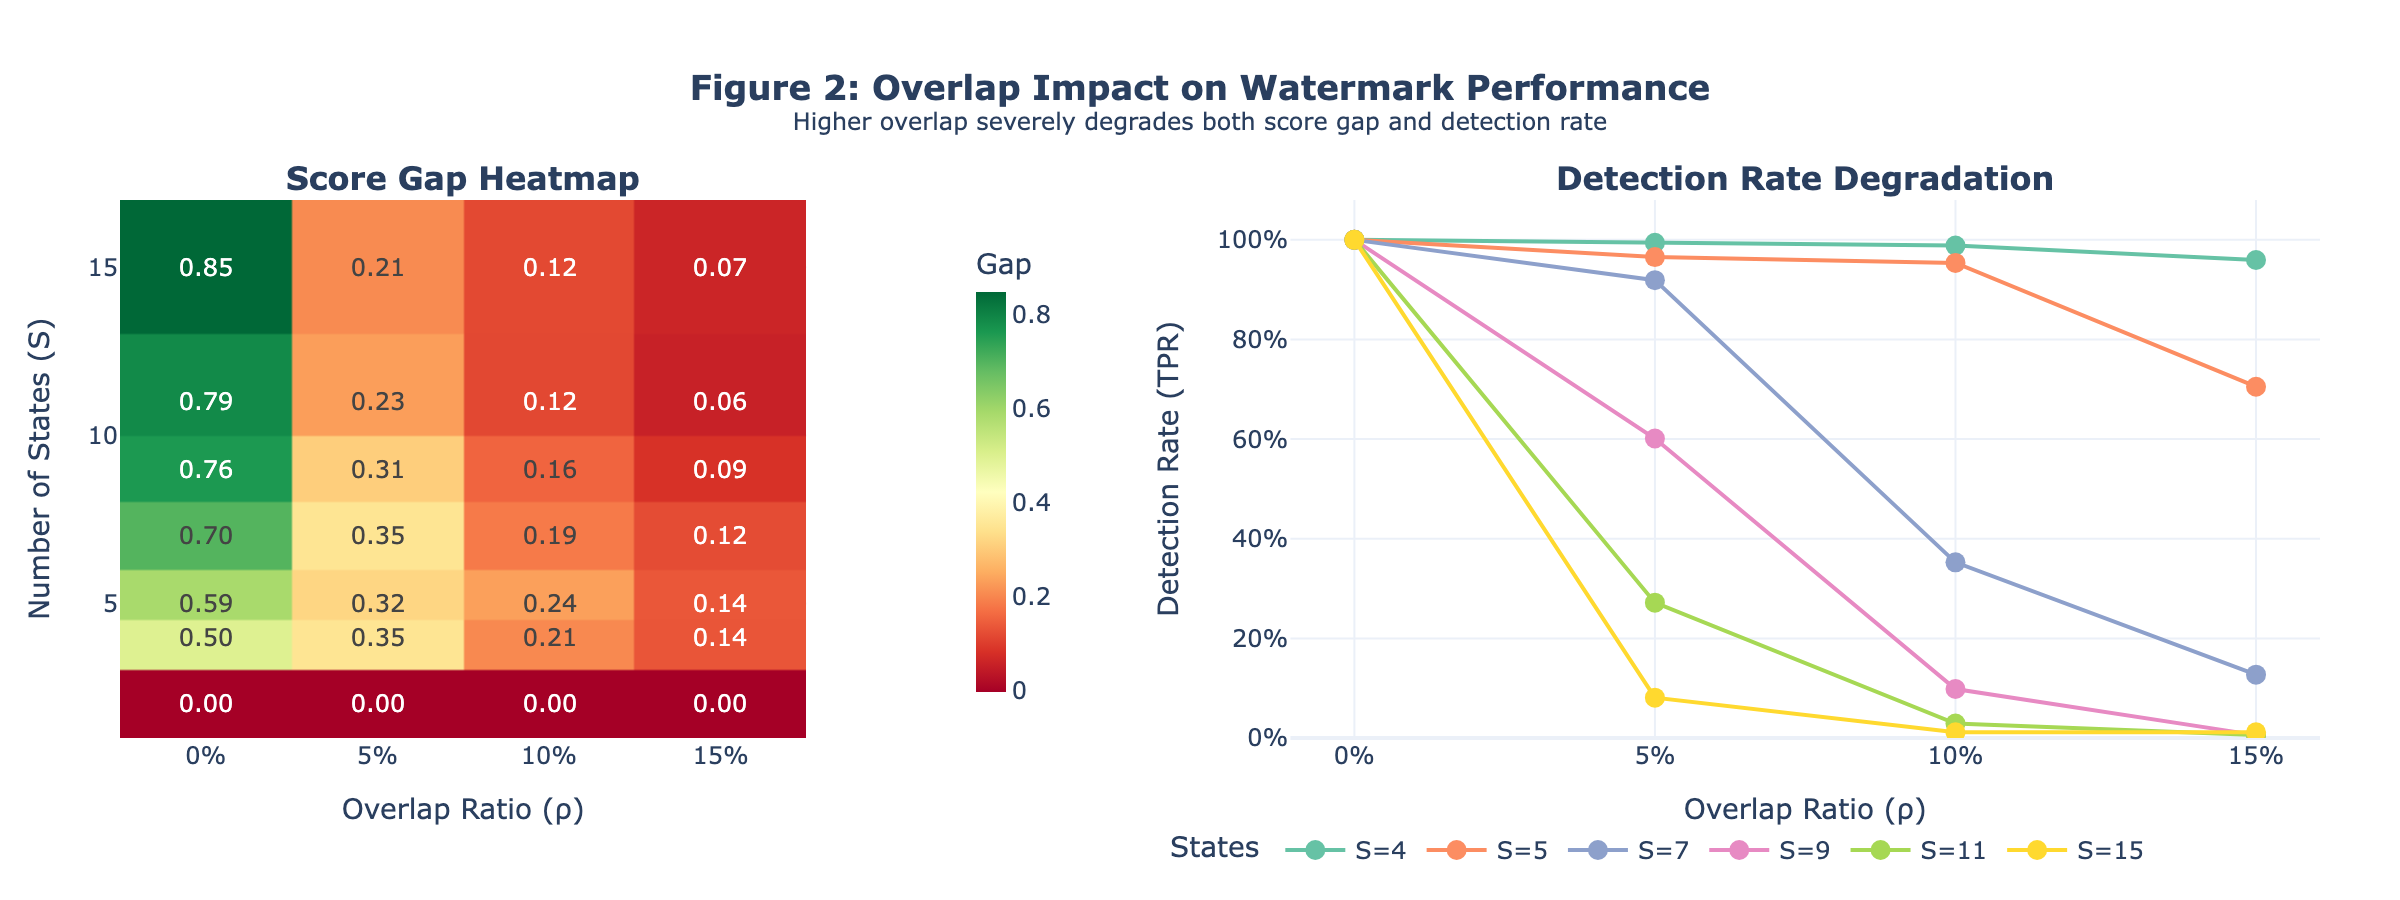
\includegraphics[width=0.95\textwidth]{pictures/fig2_overlap_impact.png}
    \caption{Overlap impact on watermark performance. \textbf{Left:} Score gap heatmap across 28 configurations---gap decreases with higher overlap and lower states. \textbf{Right:} Detection rate degradation curves showing higher state counts are more sensitive to overlap.}
    \label{fig:overlap_impact}
\end{figure}

\begin{figure}[H]
    \centering
    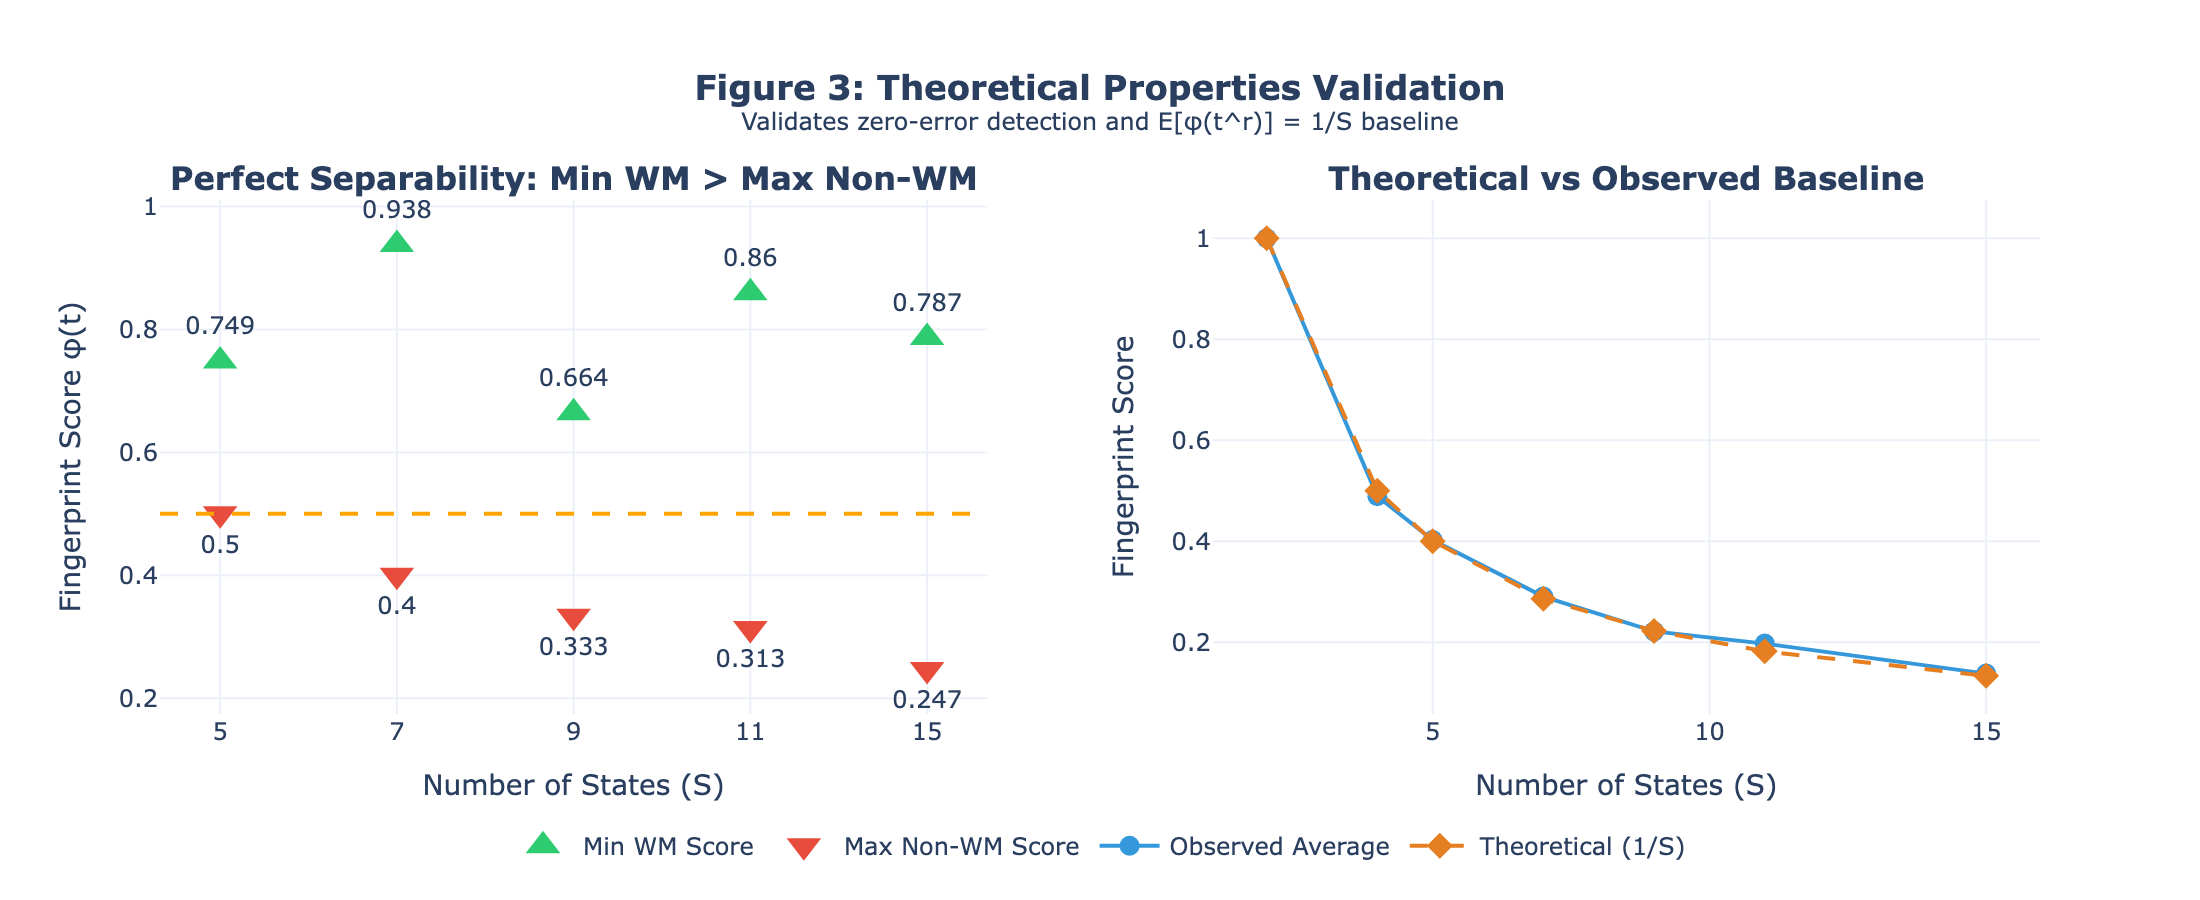
\includegraphics[width=0.95\textwidth]{pictures/fig3_theoretical.png}
    \caption{Theoretical properties validation. \textbf{Left:} Perfect separation for $S \geq 5$---minimum WM score exceeds maximum non-WM score. \textbf{Right:} Observed vs theoretical baseline $\mathbb{E}[\phi] = 1/S$, validating Theorem~\ref{thm:detection}.}
    \label{fig:theoretical}
\end{figure}

\section{Implementation Details}

\textbf{Hash function}: SHA-256 via Python \texttt{hashlib}. State assignment: \texttt{int(sha256(f"\{key\}-\{token\_id\}").hexdigest(), 16) \% S}. \textbf{Model}: meta-llama/Llama-3.2-3B-Instruct. \textbf{Generation}: greedy decoding ($T=0$), max 200 tokens. \textbf{Reproducibility}: seed 42, key \texttt{curated\_wiki\_dataset\_2024}.

% ============================================================================
% LLM USAGE STATEMENT
% ============================================================================
\section*{LLM Usage Statement}

\noindent
Claude (Anthropic) assisted with LaTeX formatting. All proofs, algorithms, and experiments independently developed and verified by the authors.

\vspace{1em}

\begin{center}
\rule{0.5\textwidth}{0.4pt}\\
\vspace{0.3em}
\textit{Template version 2.0 --- January 2026}\\
\textit{Technical AI Governance Challenge}\\
\url{https://apartresearch.com}
\end{center}

\end{document}